
\chapter{Esquema de Banco de Dados}

Devido à opção por um banco de dados não relacional, serão apresentados os esquemas de cada coleção.

\begin{figure}[htb]
	\centering
	\caption{\label{fig9_colecaousuario}Coleção de Usuário}
	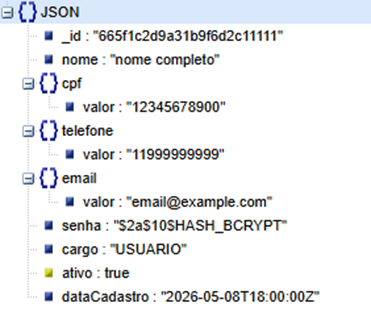
\includegraphics[scale=1.0]{images/figuras/fig9_colecao_usuario.png}
	\fonte{dos Autores}
\end{figure}

\begin{figure}[htb]
	\centering
	\caption{\label{fig10_colecao_categoria}Coleção de Categoria}
	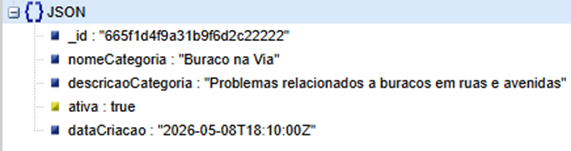
\includegraphics[scale=1.0]{images/figuras/fig10_colecao_categoria.png}
	\fonte{dos Autores}
\end{figure}

\begin{figure}[htb]
	\centering
	\caption{\label{fig11_colecao_ocorrencia}Coleção de Ocorrência}
	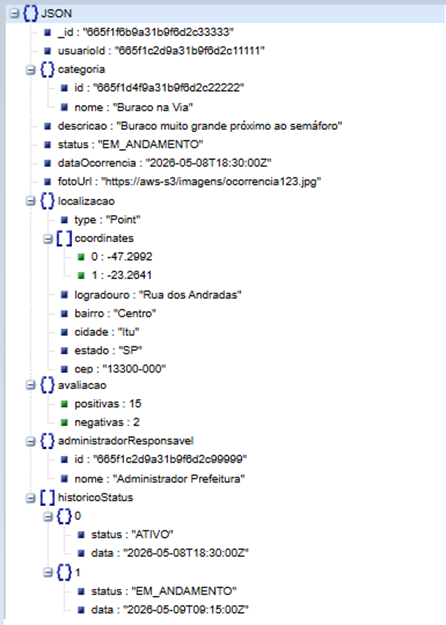
\includegraphics[scale=1.0]{images/figuras/fig11_colecao_ocorrencia.png}
	\fonte{dos Autores}
\end{figure}

\begin{figure}[htb]
	\centering
	\caption{\label{fig12_colecao_notificacao}Coleção de Notificação}
	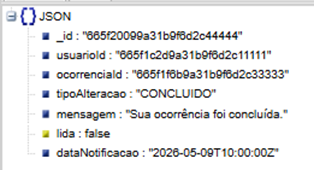
\includegraphics[scale=1.0]{images/figuras/fig12_colecao_notificacao.png}
	\fonte{dos Autores}
\end{figure}
